\documentclass[10pt,a4paper,openany,oneside]{book}

% ---------------- packages ----------------
\usepackage[margin=2cm]{geometry}
\usepackage[T1]{fontenc}
\usepackage{lmodern}
\usepackage{amsmath,amssymb}
\usepackage{graphicx}
\usepackage{booktabs}
\usepackage{xcolor}
\usepackage{listings}
\usepackage{titlesec}
\usepackage{enumitem}
\usepackage{float}
\usepackage{multicol}
\usepackage{needspace}
\usepackage[hidelinks]{hyperref}

\graphicspath{{figures/}}
\setcounter{tocdepth}{1}
\titlespacing*{\subsection}{0pt}{8pt}{2pt}

\titleformat{\chapter}[display]
  {\normalfont\Large\bfseries}{\chaptertitlename\ \thechapter}{6pt}{\LARGE}
\titlespacing*{\chapter}{0pt}{-25pt}{12pt}
\titlespacing*{\section}{0pt}{10pt}{4pt}

\setlist{nosep,leftmargin=*}

\definecolor{codegrey}{gray}{0.45}
\definecolor{codebg}{gray}{0.96}
\lstset{
  basicstyle=\ttfamily\fontsize{6.6}{7.6}\selectfont,
  backgroundcolor=\color{codebg},
  numbers=left,
  numberstyle=\tiny\color{codegrey},
  numbersep=5pt,
  keywordstyle=\bfseries\color{blue!60!black},
  commentstyle=\itshape\color{green!40!black},
  stringstyle=\color{red!60!black},
  frame=single,
  rulecolor=\color{gray!40},
  breaklines=true,
  columns=fullflexible,
  keepspaces=true,
  showstringspaces=false,
  xleftmargin=1.2em,
  framexleftmargin=1.2em,
  aboveskip=2pt,
  belowskip=4pt
}

% terminal output style
\lstdefinestyle{terminal}{
  language={},
  basicstyle=\ttfamily\fontsize{7.5}{8.6}\selectfont\color{white},
  backgroundcolor=\color{black},
  numbers=none,
  frame=single,
  rulecolor=\color{black},
  xleftmargin=0pt,
  framexleftmargin=0pt,
  framesep=6pt
}

\newcommand{\file}[1]{\texttt{#1}}
\newcommand{\lno}[1]{\par\noindent\hangindent=4.2em\hangafter=1\makebox[4.2em][l]{\textbf{#1}}}
\newcommand{\lnin}[1]{#1}
\newcommand{\code}[4]{\lstinputlisting[language=#2,firstline=#3,lastline=#4,firstnumber=#3,basicstyle=\ttfamily\footnotesize,aboveskip=6pt,belowskip=4pt]{code/#1}}

% =====================================================
\begin{document}

% ---------------- title page ----------------
\begin{titlepage}
  \centering
  \IfFileExists{image.png}{\includegraphics[width=0.20\linewidth]{image.png}\par}{}
  \vspace*{0.5cm}
  {\Large PROJECT BASED LEARNING REPORT\par}
  \vspace{1.5cm}
  {\Huge\bfseries Monte Carlo Risk Model\\[4pt] for a Stock Investment\par}
  \vspace{0.8cm}
  {\large Value at Risk, hypothesis testing,\\ correlation and regression on real market data\par}
  \vspace{2.5cm}
  {\large Submitted by\par}
  \vspace{0.3cm}
  {\large
  \begin{tabular}{ll}
    Udit Sharma & 2502030002\\
    Harshil Kumar & 2502030009\\
    Utkarsh Singh & 2502030013\\
    Shiveswar Sharma & 2502030016\\
    Kritika Naagar & 2502030022
  \end{tabular}\par}
  \vspace{1.5cm}
  {\large Under the guidance of\\[4pt] \textbf{Dr. Rupali Shrivastava}\par}
  \vfill
  {\large Department of Mathematics\\ Jaypee Institute of Information Technology\par}
  \vspace{0.4cm}
  {\large November 2026\par}
\end{titlepage}

% ---------------- abstract + contents ----------------
\section*{Abstract}

If you put money into a stock for a year, how likely are you to lose money, and how much
could you lose? We wrote a small program that answers this for any stock on Yahoo Finance.
It downloads two years of daily prices, works out the average daily return $\mu$ and the
volatility $\sigma$, and then simulates 10{,}000 possible years with the Monte Carlo
method. From these simulated years we get the 95\% Value at Risk (VaR) and the chance of
ending the year with a loss.

The simulation rests on a few assumptions: that returns are normal, that $\mu$ and
$\sigma$ stay the same over time, and that $\mu$ is a real effect and not noise. We check
each of these with the tests from sampling theory (t-test, F-test and chi-square test), and
we use correlation, least squares and regression to see how the stock moves with the
market.

For \$10{,}000 in Apple (AAPL) the 95\% VaR is \$2{,}353 and the chance of a loss is
23.1\%. The tests show that the average return is not significantly different from zero,
that the volatility changed between the two years, and that the returns are not normal.
Apple moves almost one to one with the market ($\beta = 1.02$), but the market explains
only 36\% of its daily moves. So the VaR from the simple model should be read as a lower
estimate of the real risk.

\vspace{-1em}
\begingroup
\renewcommand{\chapter}[2]{\section*{Contents}}
\tableofcontents
\endgroup

% =====================================================
\chapter{Introduction}

\section{Problem statement}
\emph{``If I invest money in a stock for one year, how likely am I to lose money, and how
much could I lose?''}
Banks and funds answer this question every day with a number called the \textbf{Value at
Risk}. A typical statement is: \emph{``there is a 5\% chance that this investment loses
more than \$2{,}353 in one year.''}

\section{Objectives}
\begin{enumerate}
  \item Download daily prices for any stock, and for the market (the S\&P~500 fund SPY).
  \item Estimate $\mu$ and $\sigma$ of the daily returns and simulate 10{,}000 years
    (Monte Carlo) to get the VaR and the chance of a loss.
  \item Use the t-test, F-test and chi-square test to check if the assumptions behind the
    simulation actually hold for the data.
  \item Use least squares, correlation and regression to measure the trend of the stock
    and how strongly it follows the market.
\end{enumerate}

\section{Scope}
The model does not predict whether a stock will go up. It describes the range of outcomes
that fit the past behaviour of the stock, and how likely the bad ones are. Chapter~2 covers
the theory, Chapter~3 explains the code line by line, Chapter~4 has the results and
Chapter~5 the conclusions. The full code is in the Appendix.

% =====================================================
\chapter{Background}

\section{Returns, mean and volatility}
We work with daily \textbf{log returns} instead of prices:
\begin{equation}
  r_t = \ln\left(P_t / P_{t-1}\right).
\end{equation}
For small moves this is almost the percentage change (\$100 to \$102 gives
$\ln 1.02 \approx 0.0198$). Log returns add up over time, so the value after $T$ days is
$P_T = P_0\, e^{\,r_1 + \dots + r_T}$. From $n$ returns we estimate
\begin{equation}
  \bar r = \mu = \frac{1}{n}\sum r_t, \qquad
  s = \sigma = \sqrt{\frac{1}{n-1}\sum (r_t-\bar r)^2 } .
\end{equation}
We divide by $n-1$ because $\bar r$ comes from the same data. Over a year of 252 trading days
the mean grows like $252\mu$ but the spread only like $\sqrt{252}\,\sigma$.

\section{Monte Carlo simulation and Value at Risk}
The Monte Carlo method~\cite{metropolis} solves a problem by simulating it many times and
counting the results. We assume each day's return is drawn from a normal distribution
$\mathcal{N}(\mu,\sigma^2)$, which is the geometric Brownian motion model of stock
prices~\cite{hull}. One simulated year is 252 such draws:
\begin{equation}
  V_{t+1} = V_t \, e^{\,r_t}, \qquad r_t \sim \mathcal{N}(\mu, \sigma^2).
\end{equation}
Doing this $N=10{,}000$ times gives $N$ possible end values $V_T$. The 95\% VaR is the loss
that is only beaten in 5\% of the years~\cite{jorion}:
\begin{equation}
  \text{VaR}_{95} = V_0 - q_{0.05}(V_T),
\end{equation}
where $q_{0.05}$ is the 5th percentile, which we read off by sorting the $N$ values. The
random numbers come from the Mersenne Twister generator~\cite{mt}, started from a fixed
seed so every run gives the same answer. The error of a Monte Carlo estimate falls like
$1/\sqrt N$, so 10{,}000 runs are accurate to about 1\%~\cite{glasserman}.

\section{Testing a hypothesis}
A test starts with a \textbf{null hypothesis} $H_0$ (``nothing special is going on'') and an
alternative $H_1$. From the sample we compute a \textbf{test statistic} and compare it with
the value from the statistical table at the \textbf{significance level} $\alpha = 0.05$. If
the statistic is bigger than the table value we reject $H_0$; otherwise we accept it. With
$\alpha=0.05$ there is a 5\% chance of rejecting a true $H_0$ (a Type~I error). The t, F
and $\chi^2$ tests are called \emph{exact} or \emph{small sample} tests because they hold
for any sample size when the data is normal, unlike the large sample $z$ test~\cite{gupta}.

\section{The t-test}
\textbf{One sample.} To test $H_0: \mu = 0$,
\begin{equation}
  t = \frac{\bar r}{s/\sqrt n}, \qquad \text{df} = n-1 .
\end{equation}
\textbf{Two samples.} To test if two samples $a$ and $b$ have the same mean, we use the
pooled variance when their variances are equal:
\begin{equation}
  s_p^2 = \frac{(n_a-1)s_a^2 + (n_b-1)s_b^2}{n_a+n_b-2},\qquad
  t = \frac{\bar a - \bar b}{s_p\sqrt{1/n_a + 1/n_b}},\qquad \text{df}=n_a+n_b-2 .
\end{equation}
When the variances are not equal we use Welch's version,
$t = (\bar a - \bar b)/\sqrt{s_a^2/n_a + s_b^2/n_b}$, with the Welch--Satterthwaite degrees
of freedom. The F-test below tells us which one to use.

\section{The F-test}
To test if two samples have the same variance, $H_0: \sigma_a^2 = \sigma_b^2$, we divide the
larger sample variance by the smaller one:
\begin{equation}
  F = s_a^2 / s_b^2, \qquad \text{df} = (n_a-1,\ n_b-1).
\end{equation}

\section{The chi-square goodness of fit test}
To test if data follows a given distribution, we split the range into $k$ bins and compare
the observed count $O_i$ in each bin with the expected count $E_i$:
\begin{equation}
  \chi^2 = \sum_{i=1}^{k} \frac{(O_i - E_i)^2}{E_i}, \qquad \text{df} = k - 1 - p ,
\end{equation}
where $p$ is the number of parameters estimated from the data. For a normal distribution we
estimate $\mu$ and $\sigma$, so $p=2$.

\section{Least squares, correlation and regression}
\textbf{Least squares} fits a line $y = a + bx$ by making $\sum (y_i - a - bx_i)^2$ as small as
possible, which gives
\begin{equation}
  b = \frac{\sum (x_i-\bar x)(y_i-\bar y)}{\sum (x_i-\bar x)^2}, \qquad a = \bar y - b\bar x .
\end{equation}
A curve like $P = e^{a+bx}$ can be fitted the same way by taking the log first,
$\ln P = a + bx$.

\textbf{Correlation} measures how closely two variables move together, from $-1$ to $+1$:
\begin{equation}
  r = \frac{\sum (x_i-\bar x)(y_i-\bar y)}{\sqrt{\sum (x_i-\bar x)^2 \sum (y_i-\bar y)^2}},
  \qquad t = \frac{r\sqrt{n-2}}{\sqrt{1-r^2}},\ \ \text{df}=n-2,
\end{equation}
where the $t$ value tests $H_0$: no correlation.

\textbf{Regression} of the stock return on the market return,
$r_{\text{stock}} = \alpha + \beta\, r_{\text{market}}$, is fitted by least squares. The slope
$\beta$ (\emph{beta}) says how much the stock moves when the market moves by 1\%. The
$R^2 = r^2$ is the share of the stock's variance explained by the market. That part is
\emph{market risk}, which cannot be removed by owning more stocks. The rest is
\emph{stock specific risk}, which can~\cite{hull}.

% =====================================================
\chapter{Methodology}

\section{How the program is organised}
The project is four small programs that pass data through text files. The
\file{Makefile} runs them in order. In this chapter each piece of code is shown with its
line numbers, followed by what those lines do. The complete files are also in the Appendix.

\begin{center}
\begin{tabular}{@{}llll@{}}
\toprule
Step & Program & Reads & Writes \\
\midrule
1. Download & \file{fetch.py} & ticker (keyboard) & \file{prices.txt}, \file{market.txt}, \file{ticker.txt} \\
2. Simulate & \file{calc.cpp} & \file{prices.txt} & \file{returns.txt}, \file{paths.txt}, \file{finals.txt}, \file{results.txt} \\
3. Plot & \file{plot.py} & output of step 2 & \file{risk.png} \\
4. Test & \file{stats.py} & \file{prices.txt}, \file{market.txt} & \file{stats.png} \\
\bottomrule
\end{tabular}
\end{center}

We used Python where libraries do most of the work (downloading, plotting, looking up
table values) and C++ for the simulation, which needs about 2.5 million random numbers. In
\file{stats.py} every statistic is computed by hand from the formulas in Chapter~2. The
\file{scipy} library is only used in place of a printed statistical table, to look up the
5\% table values.

\section{Makefile}
\code{Makefile}{make}{1}{6}
\lno{1} \texttt{run:} is the name of the target, so typing \texttt{make} runs every line under it, in order.
\lno{2} runs the download script with the Python from the project's virtual environment (\file{.venv}).
\lno{3} compiles \file{calc.cpp} with \texttt{g++} into a program called \file{calc}.
\lno{4} runs the simulation.
\lno{5} draws the simulation plots.
\lno{6} runs the statistical tests and draws their plots.

\section{fetch.py: downloading the data}
\code{fetch.py}{Python}{1}{21}
\lno{1} imports \texttt{yfinance}~\cite{yfinance}, a library that downloads data from Yahoo Finance, under the short name \texttt{yf}.
\lno{4} asks the user to type a ticker symbol, for example \texttt{AAPL} or \texttt{TSLA}.
\lno{6} downloads the last two years of daily data for the stock and keeps only the \texttt{Close} column, the price at the end of each trading day.
\lno{7} does the same for SPY, a fund that follows the S\&P~500, which we use as ``the market''.
\lno{10--11} each row is labelled with a date and a time zone. We keep only the date, so the two tables can be matched even if they come from markets in different time zones.
\lno{14} joins the two tables and keeps only the days that are in both (\texttt{how="inner"}). After this, day $t$ of the stock is the same calendar day as day $t$ of the market, which the correlation and regression need.
\lno{16--17} write the two price columns to \file{prices.txt} and \file{market.txt}. \texttt{index=False} leaves out the dates and \texttt{header=False} leaves out the column name, so each file is just one number per line, oldest first. This keeps the C++ side simple.
\lno{19} prints the table so the user can see what was downloaded.
\lno{21} saves the ticker name to \file{ticker.txt} so the plots can show it in their titles.

\section{calc.cpp: simulation and VaR}

\subsection*{Libraries and settings}
\code{calc.cpp}{C++}{1}{13}
\lno{1--6} include the parts of the C++ standard library we need: \texttt{iostream} for printing, \texttt{fstream} for reading and writing files, \texttt{vector} for lists that can grow, \texttt{cmath} for \texttt{log}, \texttt{exp} and \texttt{sqrt}, \texttt{random} for the random number generator and \texttt{algorithm} for \texttt{sort}.
\lno{8} lets us write \texttt{cout} instead of \texttt{std::cout}.
\lno{10} the whole program is inside \texttt{main}.
\lno{11--13} the three settings of the model: \$10{,}000 invested, 10{,}000 simulated years, and 252 trading days in a year (markets are closed on weekends and holidays).

\subsection*{Reading the prices}
\code{calc.cpp}{C++}{15}{21}
\lno{16} opens \file{prices.txt} for reading.
\lno{17} creates an empty list for the prices.
\lno{18} a variable that holds one price at a time.
\lno{19--21} \texttt{file >> price} reads the next number. It is true while a number could be read and false at the end of the file, so the loop runs once per line. \texttt{push\_back} adds each price to the end of the list. After the loop, \texttt{prices[0]} is the oldest price and the list holds 501 numbers.

\subsection*{Daily log returns}
\code{calc.cpp}{C++}{23}{30}
\lno{24--25} an empty list for the returns, and \file{returns.txt} opened for writing.
\lno{26} the loop starts at \texttt{i = 1} because the first day has no day before it, so 501 prices give 500 returns.
\lno{27} today's price divided by yesterday's, then the natural log. This is Equation~(2.1).
\lno{28--29} store the return in the list and also write it to the file, so \file{plot.py} can draw it.

\subsection*{Mean and standard deviation}
\code{calc.cpp}{C++}{32}{44}
\lno{33--36} add up all the returns.
\lno{37} divide by the number of returns to get $\mu$, the first part of Equation~(2.2).
\lno{40--43} for each return, take its distance from $\mu$ and square it, so that distances below and above the mean do not cancel, and add it to \texttt{total}.
\lno{44} divide by $n-1$ to get the variance and take the square root to get $\sigma$, the second part of Equation~(2.2).

\subsection*{The random number generator}
\code{calc.cpp}{C++}{46}{48}
\lno{47} creates a Mersenne Twister generator~\cite{mt} started from seed 42. The same seed always gives the same sequence of numbers, so every run gives the same result.
\lno{48} creates a normal distribution with our $\mu$ and $\sigma$. Each call \texttt{randomReturn(rng)} gives one random day that behaves, on average, like a real day of the stock.

\subsection*{The Monte Carlo loop}
\code{calc.cpp}{C++}{50}{70}
This is the main part of the project.
\lno{51--52} a list for the end value of every simulated year, and a file for the paths.
\lno{53} the outer loop runs once for every simulated year, 10{,}000 times.
\lno{54} every year starts with the full \$10{,}000.
\lno{55} the inner loop runs once for every trading day, 252 times.
\lno{56} draws a random return, turns it into a growth factor with \texttt{exp} (for example $e^{0.015} \approx 1.015$) and multiplies the money by it. This is Equation~(2.3). Repeating it 252 times gives $V_{252} = V_0\,e^{\,r_1 + \dots + r_{252}}$.
\lno{57--63} for the first 100 years only, the value after every day is written to \file{paths.txt}, one year per line. These are the lines in the middle plot. Saving all 10{,}000 years would make the file very large and the plot unreadable.
\lno{64} stores where this year ended.
\lno{67--70} write all 10{,}000 end values to \file{finals.txt} for the histogram.

\subsection*{Value at Risk and chance of a loss}
\code{calc.cpp}{C++}{72}{86}
\lno{73} sorts the end values from the worst year to the best year.
\lno{76} \texttt{sims * 5 / 100} is 500. The value at position 500 is the 5th percentile: 5\% of the years ended below it.
\lno{77} the VaR is the starting money minus that value, Equation~(2.4).
\lno{80--85} count the years that ended with less than \$10{,}000.
\lno{86} turn the count into a percentage. We write \texttt{100.0} and not \texttt{100} so that C++ does decimal division; with two whole numbers it would drop the decimals.

\subsection*{Output}
\code{calc.cpp}{C++}{88}{100}
\lno{88--92} print the results. \texttt{finals[sims / 2]} is the value in the middle of the sorted list, the median year.
\lno{94--97} save the investment, the VaR and the chance of a loss to \file{results.txt}, one per line, so \file{plot.py} knows where to draw the VaR line.
\lno{99} returning 0 tells the operating system that the program finished without errors.

\section{plot.py: the simulation plots}
\code{plot.py}{Python}{1}{22}
\lno{1--2} import \texttt{matplotlib} for plotting~\cite{matplotlib} and \texttt{numpy} for working with lists of numbers.
\lno{4--6} load the daily returns, the 100 saved years (a table of 100 rows and 252 columns) and the 10{,}000 end values.
\lno{7} loads the three numbers in \file{results.txt} into three variables at once.
\lno{8} loads the ticker name.
\lno{10--12} the three colours used in the plots.
\lno{14--18} a dark theme with a black background, a monospace font and orange titles.
\lno{20} creates one figure with three plots side by side, called \texttt{ax[0]}, \texttt{ax[1]} and \texttt{ax[2]}.
\lno{21--22} the title shows the ticker, the VaR and the chance of a loss. \texttt{:,.0f} prints a number with commas and no decimals.

\code{plot.py}{Python}{24}{46}
\lno{25--27} plot 1: a histogram of the daily returns in percent, using 60 bars.
\lno{30--31} plot 2: each of the 100 saved years is drawn as a thin line. The lines are partly see-through (\texttt{alpha=0.2}), so areas where many years overlap look brighter.
\lno{32} a dotted line at the starting money.
\lno{37} plot 3: a histogram of the 10{,}000 end values.
\lno{38} a red line at the VaR cut-off, $V_0 - \text{VaR}$. 5\% of the histogram lies to the left of it.
\lno{39} a dotted line at the starting money. Everything to the left of it is a losing year.
\lno{42} shows the legend for the two lines.
\lno{44--46} fit the plots in the window, save the figure as \file{risk.png} and show it.

\section{stats.py: the tests}

\subsection*{Data and helper functions}
\code{stats.py}{Python}{1}{29}
\lno{1--3} import the plotting library, \texttt{numpy}, and \texttt{stats} from \texttt{scipy}. We only use \texttt{scipy} to look up table values.
\lno{5--7} load the stock prices, the market prices and the ticker name.
\lno{10--11} daily log returns of the stock (\texttt{r}) and of the market (\texttt{m}). \texttt{prices[1:] / prices[:-1]} divides every price by the price before it in one step, which is the same loop as in \file{calc.cpp}.
\lno{12} \texttt{n} is the number of returns, 500.
\lno{15--20} our own mean and variance functions, written straight from Equation~(2.2), so that every statistic below is computed by us and not by a library.
\lno{23--26} compare a test statistic with its table value. If it is bigger we reject $H_0$, otherwise we accept it.
\lno{29} prints the ticker and the number of returns.

\subsection*{Test 1: one sample t-test}
\code{stats.py}{Python}{31}{40}
\lno{32} the t statistic of Equation~(2.5): the mean divided by its standard error $s/\sqrt n$.
\lno{33} the table value for a two-sided test at 5\%, which is the 97.5\% point of the t distribution with $n-1$ degrees of freedom. This is the number we would otherwise read from a t table.
\lno{34--35} print the result and the decision.
\lno{38--40} split the 500 returns into the first year (\texttt{a}) and the second year (\texttt{b}). Tests 2 and 3 compare these two years to see if the stock behaved the same way in both.

\subsection*{Test 2: F-test}
\code{stats.py}{Python}{42}{50}
\lno{43--46} divide the larger variance by the smaller one, Equation~(2.7), so that $F$ is always at least 1.
\lno{47} the table value of the F distribution with $(n_a-1, n_b-1)$ degrees of freedom.
\lno{48} remembers whether the two variances can be treated as equal. Test 3 uses this to choose its formula.
\lno{49--50} print the result.

\subsection*{Test 3: two sample t-test}
\code{stats.py}{Python}{52}{66}
\lno{53--54} the size of each sample.
\lno{55--58} if the F-test accepted equal variances, we use the pooled variance $s_p^2$ and the t statistic of Equation~(2.6), with $n_a+n_b-2$ degrees of freedom.
\lno{59--63} otherwise we use Welch's formula, which does not assume equal variances. Line 63 is the Welch--Satterthwaite formula for its degrees of freedom.
\lno{64--66} look up the table value and print the result.

\subsection*{Test 4: chi-square test}
\code{stats.py}{Python}{68}{76}
\lno{69} we use $k=10$ bins.
\lno{70} \texttt{stats.norm.ppf} cuts the normal curve with our $\mu$ and $\sigma$ into 10 pieces that each hold 10\% of the area. If the returns are normal, each bin should get 10\% of them.
\lno{71} \texttt{np.histogram} counts how many returns actually fall in each bin. These are the observed counts $O_i$.
\lno{72} the expected count in every bin, $E_i = 500/10 = 50$.
\lno{73} Equation~(2.8).
\lno{74} the table value with $\text{df} = 10 - 1 - 2 = 7$, because $\mu$ and $\sigma$ were estimated from the data. Only large values of $\chi^2$ count against $H_0$, so we use the 95\% point.

\subsection*{Least squares trend curve}
\code{stats.py}{Python}{78}{85}
\lno{79} the day numbers $0, 1, 2, \dots$ are $x$.
\lno{80} the log of the price is $y$. Taking the log turns the curve $P = e^{a+bx}$ into the straight line $\ln P = a + bx$.
\lno{81--82} the least squares slope $b$ and intercept $a$ from Equation~(2.9).
\lno{83} turns the line back into a price curve for the plot.
\lno{84--85} print $a$, $b$ and the growth of the trend over one year, $e^{252b} - 1$.

\subsection*{Correlation}
\code{stats.py}{Python}{87}{92}
\lno{88} the correlation $r$ between the stock and market returns, Equation~(2.10).
\lno{89} the t statistic that tests $H_0$: no correlation.
\lno{90} its table value with $n-2$ degrees of freedom.
\lno{91--92} print the result.

\subsection*{Regression}
\code{stats.py}{Python}{94}{99}
\lno{95} the least squares slope of stock returns on market returns. This is $\beta$, the same formula as line 81 with the market return as $x$.
\lno{96} the intercept $\alpha$.
\lno{97--99} print $\alpha$, $\beta$ and $R^2 = r^2$, the share of the stock's daily moves that the market explains.

\subsection*{Plots}
\code{stats.py}{Python}{101}{139}
\lno{102--112} the same dark theme as \file{plot.py}, and a figure with three plots whose title shows $\beta$, $r$ and $\chi^2$.
\lno{115--119} plot 1: the price and the least squares trend curve.
\lno{122} plot 2: a scatter plot with one dot per day, market return across and stock return up.
\lno{123--124} the regression line $\alpha + \beta x$, drawn between the smallest and largest market return.
\lno{125--128} titles, axis labels and the legend.
\lno{131--132} plot 3: the observed count (blue) and the expected count (red) for each of the 10 bins, side by side.
\lno{133--135} title, label and legend.
\lno{137--139} save the figure as \file{stats.png} and show it.

% =====================================================
\chapter{Results}

We used daily closing prices from 21 November 2024 to 20 November 2026 (501 days, 500
returns), \$10{,}000 invested, 10{,}000 simulated years and seed 42. The output below is
what the program prints for Apple (AAPL).

\lstinputlisting[style=terminal]{code/output.txt}

\section{Monte Carlo and Value at Risk}

\begin{figure}[H]
  \centering
  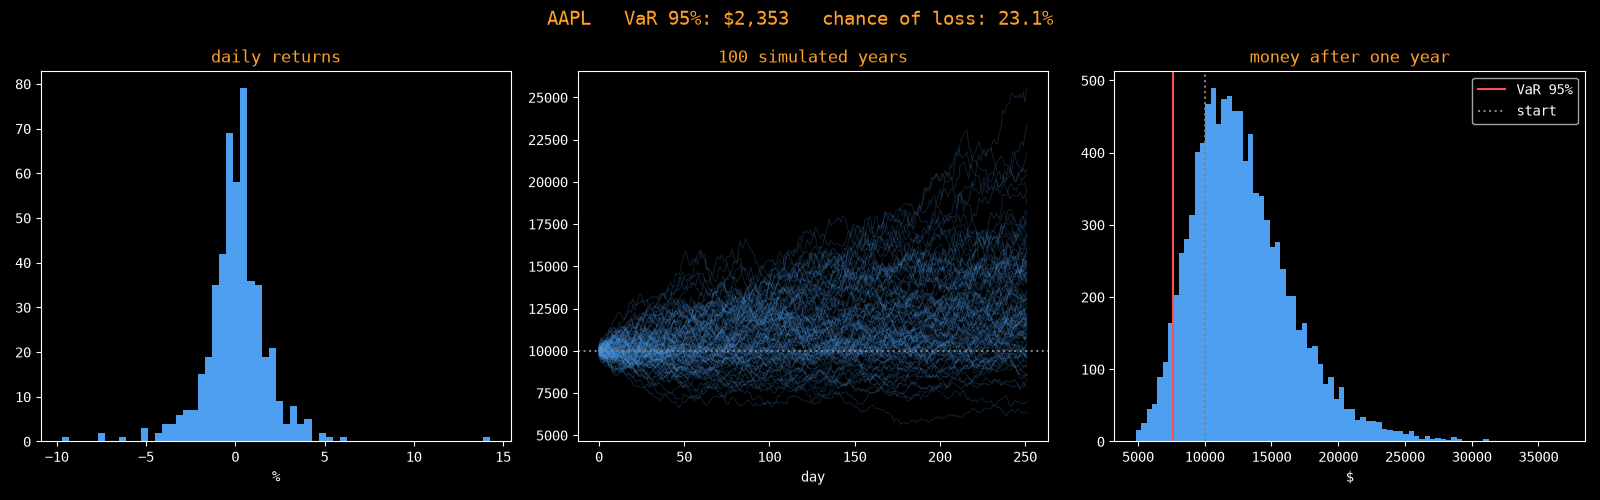
\includegraphics[width=\textwidth]{aapl_risk.png}
  \caption{AAPL: real daily returns (left), 100 of the 10{,}000 simulated years (middle), and
  the money after one year with the 95\% VaR line (right).}
  \label{fig:risk}
\end{figure}

For AAPL, $\mu = 0.0826\%$ and $\sigma = 1.82\%$ per day, which is a yearly drift of 20.8\%
and a yearly volatility of 28.9\%. The middle year ends at \$12{,}283, about one year in four
ends with a loss (23.1\%), and in one year out of twenty the loss is more than \$2{,}353. The
right plot in Figure~\ref{fig:risk} leans to the right because the money is multiplied each
day: it can never fall below zero, but it can grow a lot.

As a check, the sum of 252 normal returns is itself normal, so the VaR can also be worked
out directly: $V_0\,(1 - e^{\,252\mu - 1.645\sqrt{252}\,\sigma}) = \$2{,}345$. The simulation
gave \$2{,}353, a difference of 0.3\%, which is inside the expected Monte Carlo error.

For Tesla (TSLA) the same \$10{,}000 gives a VaR of \$6{,}029 and a 49.7\% chance of a loss.
Its daily $\sigma$ (3.56\%) is about twice Apple's and its $\mu$ is almost zero, so losing
money is close to a coin flip.

\section{Hypothesis tests and regression}

\begin{figure}[H]
  \centering
  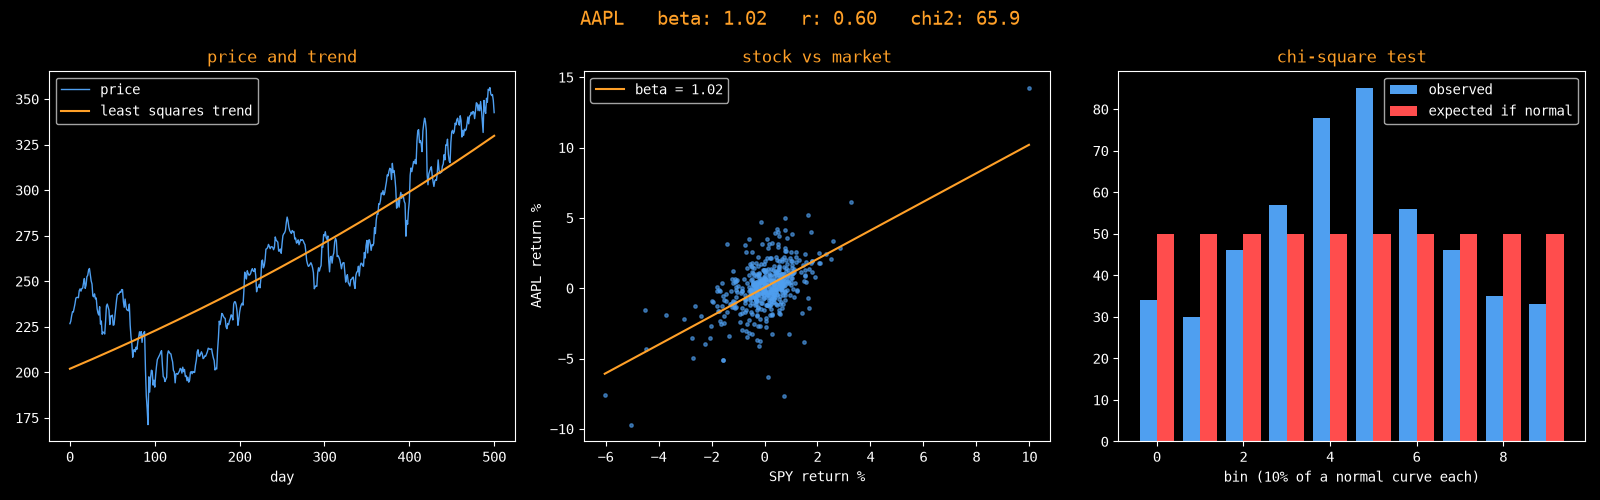
\includegraphics[width=\textwidth]{aapl_stats.png}
  \caption{AAPL: price with the least squares trend (left), daily AAPL returns against SPY
  returns with the regression line (middle), and the chi-square test (right).}
  \label{fig:stats}
\end{figure}

\begin{table}[H]
\centering
\begin{tabular}{@{}llrrrl@{}}
\toprule
Test & $H_0$ & Statistic & df & Table (5\%) & AAPL decision \\
\midrule
t-test & $\mu = 0$ & $t = 1.014$ & 499 & 1.965 & accept \\
F-test & $\sigma^2_{\text{year 1}} = \sigma^2_{\text{year 2}}$ & $F = 1.677$ & (249, 249) & 1.283 & reject \\
t-test (Welch) & $\mu_{\text{year 1}} = \mu_{\text{year 2}}$ & $t = -0.145$ & 468 & 1.965 & accept \\
$\chi^2$ test & returns are normal & $\chi^2 = 65.92$ & 7 & 14.07 & reject \\
Correlation & $\rho = 0$ & $t = 16.82$ & 498 & 1.965 & reject \\
\bottomrule
\end{tabular}
\caption{Results of the tests for AAPL at $\alpha = 0.05$. For TSLA the decisions are the same
($t=0.023$, $F=1.947$, $t=0.331$, $\chi^2=20.44$, correlation $t=19.77$).}
\label{tab:tests}
\end{table}

\textbf{The average return is not significant.} With $t = 1.014 < 1.965$ we cannot say that
Apple's average daily return is different from zero. A 21\% yearly drift sounds large, but the
daily moves are so noisy that two years of data cannot tell it apart from luck. This matters for
the simulation: if we set $\mu = 0$, the VaR becomes $V_0(1-e^{-1.645 \times 0.289}) = \$3{,}782$
instead of \$2{,}353. So a big part of the low VaR comes from a drift that we cannot prove.

\textbf{The risk changed between the two years.} $F = 1.677 > 1.283$, so the variance in the two
years was not the same. The simulation assumes one fixed $\sigma$, so its VaR depends on which
period we happen to use. Because the variances differ, the program used Welch's t-test for the
means, which found no difference ($t=-0.145$).

\textbf{The returns are not normal.} $\chi^2 = 65.92$ is far above 14.07. The right plot of
Figure~\ref{fig:stats} shows why: the middle bins hold up to 85 returns where 50 are expected, so
there are too many quiet days. The real returns are more peaked than a bell curve, and
the left plot of Figure~\ref{fig:risk} also shows a few very large days ($-9.7\%$ and $+14.3\%$)
that a normal curve almost never produces. This is the \emph{fat tails} effect described by
Mandelbrot~\cite{mandelbrot}, and it means real crashes are more likely than our model says.

\textbf{Trend.} The least squares curve gives a growth of 28.1\% per year, higher than the 23\%
($e^{0.208}-1$) from the mean return. The mean log return only depends on the first and the last
price, since the sum telescopes to $\ln(P_n/P_0)$, while least squares uses every price in between.

\textbf{Correlation and regression.} Apple and SPY have $r = 0.60$, which is clearly significant.
The regression gives $\beta = 1.02$, so Apple moves almost one to one with the market. But
$R^2 = 0.36$, so only 36\% of Apple's daily moves come from the market and 64\% are specific to
Apple. That 64\% is the part that could be reduced by owning more stocks. Tesla has
$\beta = 2.19$ and $R^2 = 0.44$: when the market falls 1\%, Tesla falls about 2.2\% on average.

% =====================================================
\chapter{Conclusions}

We built a Monte Carlo risk model that works for any stock. For \$10{,}000 in Apple it gives a
95\% VaR of \$2{,}353 and a 23.1\% chance of a loss over one year, and the simulation matches the
exact formula to 0.3\%. We then tested the assumptions behind the model. The t-test showed that
the average return is not significant, the F-test showed that the volatility is not constant, and
the chi-square test showed that the returns are not normal. Regression showed that Apple follows
the market with $\beta \approx 1$, but most of its daily movement is specific to Apple.

Put together, these results say the simple model gives a useful first number, but the real risk
is probably higher than \$2{,}353. Possible next steps are to simulate with $\mu = 0$ or with a
range of $\mu$ values, to draw returns from the real past days instead of a normal curve (so the
fat tails are kept), to simulate a portfolio of several correlated stocks, and to backtest the
VaR against what actually happened in later years.

% ---------------- references (same page) ----------------
\begingroup
\renewcommand{\chapter}[2]{\section*{References}\addcontentsline{toc}{chapter}{References}}
\begin{thebibliography}{9}
\small
\bibitem{hull} J.~C. Hull, \emph{Options, Futures, and Other Derivatives}, 10th ed. Pearson, 2018.
\bibitem{jorion} P.~Jorion, \emph{Value at Risk: The New Benchmark for Managing Financial Risk},
  3rd ed. McGraw-Hill, 2006.
\bibitem{glasserman} P.~Glasserman, \emph{Monte Carlo Methods in Financial Engineering}.
  Springer, 2003.
\bibitem{metropolis} N.~Metropolis and S.~Ulam, ``The Monte Carlo method,'' \emph{Journal of the
  American Statistical Association}, vol.~44, no.~247, pp.~335--341, 1949.
\bibitem{mandelbrot} B.~Mandelbrot, ``The variation of certain speculative prices,'' \emph{The
  Journal of Business}, vol.~36, no.~4, pp.~394--419, 1963.
\bibitem{mt} M.~Matsumoto and T.~Nishimura, ``Mersenne Twister: a 623-dimensionally
  equidistributed uniform pseudo-random number generator,'' \emph{ACM Trans. on Modeling and
  Computer Simulation}, vol.~8, no.~1, pp.~3--30, 1998.
\bibitem{gupta} S.~C. Gupta and V.~K. Kapoor, \emph{Fundamentals of Mathematical Statistics},
  Sultan Chand \& Sons, 2020.
\bibitem{matplotlib} J.~D. Hunter, ``Matplotlib: A 2D graphics environment,'' \emph{Computing in
  Science \& Engineering}, vol.~9, no.~3, pp.~90--95, 2007.
\bibitem{yfinance} R.~Aroussi, \emph{yfinance}. \url{https://github.com/ranaroussi/yfinance}
\end{thebibliography}
\endgroup

% =====================================================
\appendix
\titlespacing*{\chapter}{0pt}{-30pt}{8pt}
\chapter{Source Code}
\vspace{-12pt}
\begin{multicols}{2}
\noindent\textbf{\file{calc.cpp}}
\lstinputlisting[language=C++]{code/calc.cpp}

\noindent\textbf{\file{Makefile}}
\lstinputlisting[language=make]{code/Makefile}

\noindent\textbf{\file{fetch.py}}
\lstinputlisting[language=Python]{code/fetch.py}

\noindent\textbf{\file{plot.py}}
\lstinputlisting[language=Python]{code/plot.py}

\noindent\textbf{\file{stats.py}}
\lstinputlisting[language=Python]{code/stats.py}
\end{multicols}

\end{document}
